
\chapter{\'Etudes de cas et exp\'erimentations~: Comparaisons de \ppff\ avec Java et FastFlow}
\label{experiences.chap}


Ce chapitre pr\'esente une \'evaluation exp\'erimentale de \TT{PpFf} afin de comparer ses performances avec d'autres approches d'ex\'ecution parall\`ele, plus sp\'ecifiquement avec \TT{Java} et \TT{FastFlow}.
%
Dans les sections~\ref{wordcount.sect} et~\ref{stockprice.sect}, nous pr\'esentons deux applications \'ecrites avec \PpFf. Ces applications ont \'et\'e choisies non seulement pour montrer certaines fonctionnalit\'es de l'API, mais \'egalement pour leur pertinence dans des sc\'enarios typiques. La section~\ref{wordcount.sect} pr\'esente une application permettant de calculer le nombre d'occurrences des mots dans un texte --- le <<\emph{Hello World!}>> des syst\`emes de traitement de donn\'ees en mode \emph{batch} --- alors que la section~\ref{stockprice.sect} pr\'esente une application permettant de calculer des statistiques sur les prix d'indices boursiers --- un exemple typique de traitement de flux en ligne (\emph{online data processing}). Mais tout d'abord, nous pr\'esentons la fa\c{c}on dont nos exp\'erimentations ont \'et\'e effectu\'ees.

%Finalement, la section~\ref{coutsPpFf.sect} pr\'esente une application permettant de d\'eterminer les surco\^uts introduits par \TT{PpFf} par rapport \`a \TT{FastFlow} --- un \emph{micro benchmark} consistant en un pipeline avec un seul op\'erateur. 



\section{M\'ethode utilis\'ee pour les exp\'erimentations}
\label{usedMethodsForBenchmarks.chap}

Chaque syst\`eme informatique a des caract\'eristiques propres. Les principaux facteurs qui influencent les performances d'un tel syst\`eme sont le type de processeur, le nombre de processeurs ou de c\oe{}urs, et le r\'eseau de communication. 



\goodbreak
\begin{samepage}
Afin d'avoir des r\'esultats plus g\'en\'eraux, nous avons conduit nos exp\'eriences sur les machines suivantes~:
\label{machines.sect}


\begin{description}
\item[\M1] = \TT{java.labunix.uqam.ca}~: Une machine avec 16 processeurs de 2,6 GHz, chacun contenant 6 cœurs. Le syst\`eme d'exploitation est Linux version 3.10.0. 


\item[\M2] = \TT{japet.labunix.uqam.ca}~:  Une machine avec 64 processeurs de 2,3 GHz, chacun contenant 8 cœurs. Le système d'exploitation est Linux version 3.10.0.

\item[\M3] = \TT{c34581}~:  Une machine avec 8 processeurs de 3,6 GHz, chacun contenant 4 cœurs. Le système d'exploitation est Linux.


\end{description}
\end{samepage}

\newcommand{\LARGEUR}{3cm}

\begin{table}
\begin{tabular}{|p{3cm}|p{\LARGEUR}|p{\LARGEUR}|p{\LARGEUR}|}
\hline
  & \M1 & \M2 & \M3
\\\hline
\textbf{OS} & CentOS 7.8.2003 & CentOS 7.8.2003 & CentOS 7.6.1810
\\\hline
\textbf{Mono/multi-usager} & Multi & Multi & Mono
\\\hline
\textbf{Nb.~coeurs physiques} & 16 & 32 & 4
\\\hline
\textbf{Nb.~coeurs logiques} & 16 & 64 & 8
\\\hline
\texttt{java}
  & \texttt{openjdk 11.0.7 2020-04-14 LTS}
  & \texttt{java version "1.8.0\_51"}
  & \texttt{openjdk version "11.0.7" 2020-04-14 LTS}
\\\hline
\texttt{g++ (GCC)}
   & 8.3.1
   & 8.3.1 
   & 8.3.0
\\\hline
\end{tabular}
\caption{Blah, blah}
\label{machines.table}
\end{table}




Les machines \M1 et \M2 sont des machines multi-usagers, tandis que la machine \M3 est une machine mono-usager sur laquelle les exp\'eriences ont \'et\/e roul\'ees sans interf\'erence.

Le fonctionnement des programmes \TT{Java} et~\TT{PpFf} n'est pas le m\^eme. Alors que \TT{PpFf} permet de varier le nombre de fils d'ex\'ecution (\emph{threads}), \TT{Java} ne le permet pas. Afin de montrer les meilleurs temps d'ex\'ecution et l'\'evolutivit\'e de \TT{PpFf}, des exp\'eriences pr\'eliminaires ont \'et\'e effectu\'ees, sur chaque machine, pour identifier les meilleures versions. Les exp\'eriences pr\'eliminaires ont \'et\'e conduites avec un nombre de r\'ep\'etitions de 10 et avec une quantit\'e moyenne de donn\'ees. 

Dans le cas de \TT{PpFf} et \TT{FastFlow}, l'objectif \'etait de d\'eterminer le meilleur niveau de parall\'elisme \`a utiliser dans les \TT{farm}, par exemple, pour \TT{PpFf}, la valeur pour la m\'ethode \TT{parallel()}, pour le parall\'elisme de donn\'ees. Cependant, dans tous les cas, pour \TT{Java}, c'\'etait la version avec \TT{warmup} qui a \'et\'e utilis\'ee.

L'effet de pr\'echauffage (\TT{warmup} en anglais) est g\'en\'eralement d\^u au chargement des classes et \`a l'interpr\'etation des \TT{bytecodes} au d\'emarrage du programme. Chaque fois qu'une nouvelle application d\'emarre, toutes les classes requises sont charg\'ees en m\'emoire par le mod\`ele de chargement paresseux (\TT{lazy loading} en anglais). Ce mod\`ele de conception est un mod\`ele couramment utilis\'e en programmation informatique pour reporter l'initialisation d'un objet jusqu'au point o\`u il est n\'ecessaire. Le premier appel \`a une application \TT{Java} est souvent beaucoup plus lent que le temps de r\'eponse moyen pendant la dur\'ee de vie du processus. Cette p\'eriode de pr\'echauffage est g\'en\'eralement attribu\'ee au chargement de classe paresseux et à la compilation \emph{JIT} (\emph{Just-In-Time compiler}).    

\label{jitDescription.sect}
\emph{JIT}~\citep{cramer1997compiling} est un composant de l'environnement d'ex\'ecution Java qui am\'eliore les performances des applications en compilant le \emph{bytecode} de la machine virtuelle en code machine \emph{au moment de l'ex\'ecution}. Le \emph{bytecode} est l'ensemble des instructions de la \emph{JVM} (\emph{Java Virtual Machine}) qui permet aux applications d'\^etre ex\'ecut\'ees sur plusieurs plates-formes. La conversion du \emph{bytecode} en langage machine a un impact significatif sur la vitesse d'ex\'ecution.

Dans toutes nos exp\'eriences, les programmes \TT{Java} ont \'et\'e pr\'echauff\'es en lancent une proc\'edure de pr\'echauffage avant d'ex\'ecuter les exp\'eriences mesur\'ees. La proc\'edure de pr\'echauffage consiste d'un appel \`a toutes les m\'ethodes utilis\'ees dans les exp\'eriences. Ce m\'ecanisme nous permet de charg\'ees en m\'emoire toutes les classes ce qui les rend accessibles plus rapidement pendant l'ex\'ecution d'exp\'eriences.
 
Il faut noter que le temps mesur\'e dans toutes les exp\'eriences exclut le lancement du programme. La mesure du temps se fait de l'int\'erieur du programme m\^eme, une fois celui-ci lanc\'e. Lorsque le traitement est termin\'e, le temps est \'emis en sortie du programme sur \TT{stdout}. Donc, le temps n'est pas mesur\'e avec la commande << time >>. Notamment, dans le cas de \TT{Java}, cela exclut le temps de lancement de la machine virtuelle. De plus les quantit\'es de donn\'ees utilis\'ees dans exp\'eriences ont \'et\'e restreint de sorte que le temps d'ex\'ecution soit d'au moins 225 millisecondes. Cela nous a permis d'avoir une meilleure visibilit\'e sue les performances obtenues par les trois programmes. 

Afin de montrer les \'etapes d'exp\'eriences qui ont conduit aux r\'esultats finaux, l'annexe~\ref{ExperiencesPreliminairesWordCount} pr\'esent le fichier de configuration -- \TT{WordCount-bm-config.rb} -- utilis\'e pour l'ex\'ecution des tests et quelques r\'esultats obtenus. Cr\'e\'e par mon directeur de recherche, ce fichier nous permet de configurer en avance les tests \`a ex\'ecuter. Dans ce fichier on peut sp\'ecifier tous les param\`etres dont on a besoin : le nom de la machine, les donn\'ees, le nombre de r\'ep\'etitions, et les programmes \`a ex\'ecuter. Les donn\'ees sont regroup\'ees par taille en trois cat\'egories : donnees-preliminaires, pas-mal-de-donnees et beaucoup-de-donnees. Les deux premi\`eres cat\'egories ont servi pour d\'eterminer les meilleures versions \`a utiliser. Par exemple le premier graphe montre les temps d'ex\'ecution pour \TT{WordCount} sur la machine \M1 pour le programme \TT{PpFf} en utilisant la premi\`ere cat\'egorie de donn\'ees. Les temps sont en millisecondes (ms), obtenus en prenant la moyenne de 10 ex\'ecutions.  En utilisant le fichier mentionn\'e ci-dessus, trois s\'eries de tests ont \'et\'e effectu\'ees : \TT{PpFf-1} avec un \TT{thread}, \TT{PpFf-2} avec deux \TT{threads} et \TT{PpFf-3} avec trois \TT{threads}. 

L'objectif de ces tests pr\'eliminaires est de d\'eterminer la valeur optimale pour les temps d'ex\'ecution. On peut observer que le temps d'ex\'ecution pour \TT{PpFf-3} est beaucoup plus grand que les autres deux s\'eries de tests. Il nous reste \`a d\'eterminer le meilleur temps d'ex\'ecution en comparant les deux derni\`eres s\'eries de tests.

Pour mieux distinguer les performances entre les deux s\'eries de tests, une seconde unit\'e de mesure a \'et\'e utilis\'ee : log ms. Montr\'e dans le deuxi\`eme graphe de la m\^eme annexe, on peut observer que \TT{PpFf-2} avec 2 \TT{threads} est plus performant que \TT{PpFf-1} avec un seul \TT{thread}. 

\TT{PpFf-2} est la version qui sera compar\'ee aux autres programmes lors des tests finaux. Ces tests finaux comparent les meilleures versions entre elles, en utilisant de plus grandes quantit\'es de donn\'ees et 30 r\'ep\'etitions.


\section{Analyse de l'application \TT{WordCount}}
\label{wordcount.sect}



\subsection{Description de l'application \TT{WordCount}}


Dans la section.~\ref{descriptionWordCount.sect}, nous avons pr\'esent\'e \TT{WordCount}, une application simple qui compte le nombre d'occurrences des divers mots dans un fichier texte. L'application prend en entr\'ee un fichier texte et produit un conteneur de type \TT{map<string, int>} où la cl\'e repr\'esente un mot dans le fichier et la valeur  type \TT{int}  associ\'ee repr\'esente le nombre d'occurrences du mot dans le fichier. Le code source des applications \TT{WordCount} en~\TT{PpFf} et~\TT{Java} est pr\'esent\'e dans les annexes~\ref{sourceCodeWordCountPpFf.ann} et~\ref{sourceCodeWordCountJava.ann} respectivement.


\subsection{Mesures obtenues et analyse des r\'esultats}

\graphe{WordCount-temps-java-500-30}{Programmes Seq, Java, PpFf et FastFlow}
\graphe{WordCount-debits-java-500-30}{Programmes Seq, Java, PpFf et FastFlow}

\graphe{WordCount-temps-japet-600-30}{Programmes Seq, Java, PpFf et FastFlow}
\graphe{WordCount-debits-japet-600-30}{Programmes Seq, Java, PpFf et FastFlow}

\graphe{WordCount-temps-c34581-400-30}{Programmes Seq, Java, PpFf et FastFlow}
\graphe{WordCount-debits-c34581-400-30}{Programmes Seq, Java, PpFf et FastFlow}

%
%\begin{figure}
%\centering
%     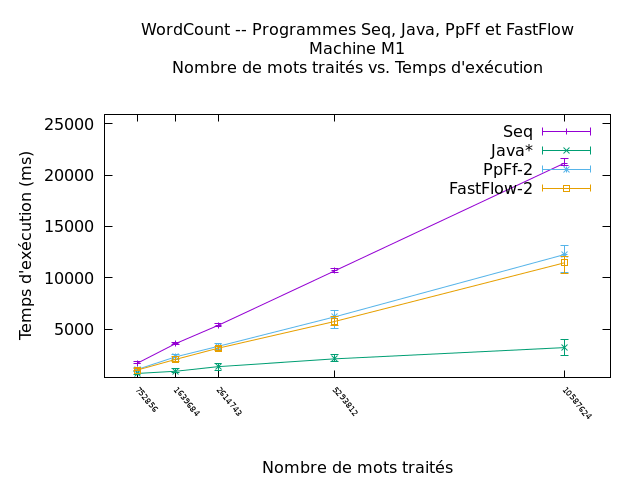
\includegraphics[width=1.0\textwidth]{Figures/WordCount-temps-java-500-30.png}
%      \caption[Les temps d'ex\'ecution pour \TT{WordCount} sur la machine \M1.]{Les temps d'ex\'ecution pour \TT{WordCount} sur la machine \M1, pour les programmes \TT{Seq}, \TT{Java}, \TT{PpFf} et \TT{FastFlow}. Les temps sont en millisecondes (ms), obtenus en prenant la moyenne de 30 ex\'ecutions.}
%       \label{GrapheTempsWordCountJava.fig}
%\end{figure}
%
%\begin{figure}
%\centering
%     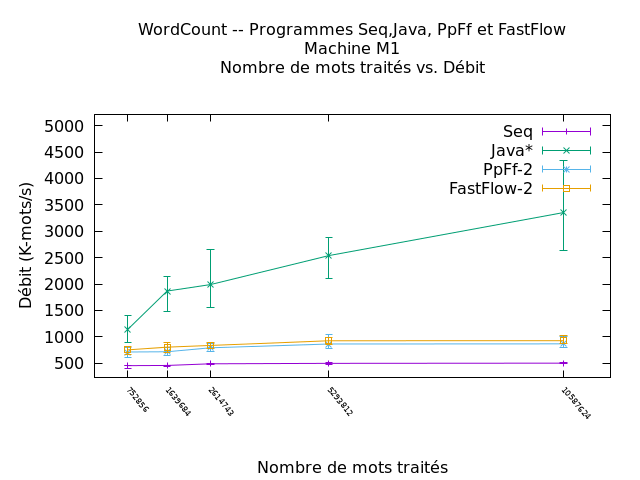
\includegraphics[width=1.0\textwidth]{Figures/WordCount-debits-java-500-30.png}
%      \caption[Les d\'ebits pour \TT{WordCount} sur la machine \M1.]{Les d\'ebits pour \TT{WordCount} sur la machine \M1, pour les programmes \TT{Seq}, \TT{Java}, \TT{PpFf} et \TT{FastFlow}. Les d\'ebits sont en milliers de mots par seconde (K-mots/s), obtenus en prenant la moyenne de 30 ex\'ecutions.}
%       \label{GrapheDebitsWordCountJava.fig}
%\end{figure}
%
%\begin{figure}
%\centering
%     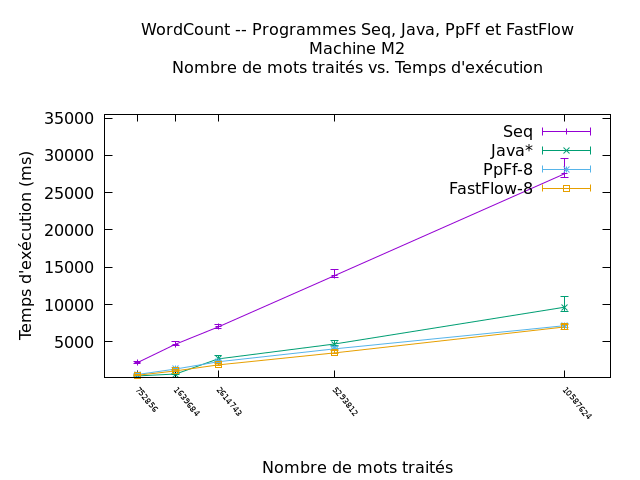
\includegraphics[width=1.0\textwidth]{Figures/WordCount-temps-japet-600-30.png}
%      \caption[Les temps d'ex\'ecution pour \TT{WordCount} sur la machine \M2.]{Les temps d'ex\'ecution pour \TT{WordCount} sur la machine \M2, pour les programmes \TT{Seq}, \TT{Java}, \TT{PpFf} et \TT{FastFlow}. Les temps sont en millisecondes (ms), obtenus en prenant la moyenne de 30 ex\'ecutions.}
%       \label{GrapheTempsWordCountJapet.fig}
%\end{figure}
%
%\begin{figure}
%\centering
%     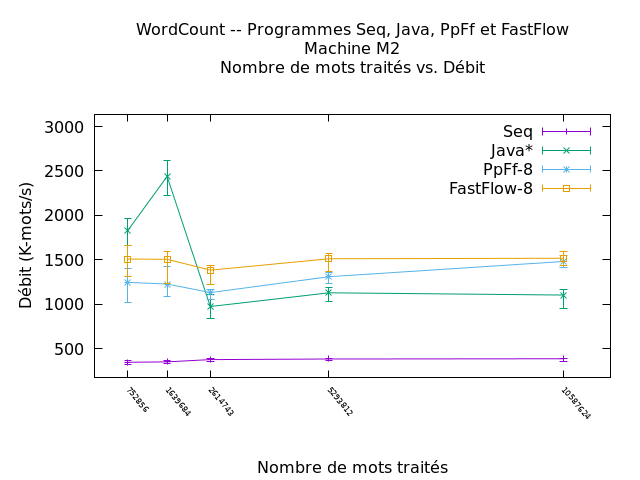
\includegraphics[width=1.0\textwidth]{Figures/WordCount-debits-japet-600-30.png}
%      \caption[Les d\'ebits pour \TT{WordCount} sur la machine \M2.]{Les d\'ebits pour \TT{WordCount} sur la machine \M2, pour les programmes \TT{Seq}, \TT{Java}, \TT{PpFf} et \TT{FastFlow}. Les d\'ebits sont en milliers de mots par seconde (K-mots/s), obtenus en prenant la moyenne de 30 ex\'ecutions.}
%       \label{GrapheDebitsWordCountJapet.fig}
%\end{figure}
%
%\begin{figure}
%\centering
%     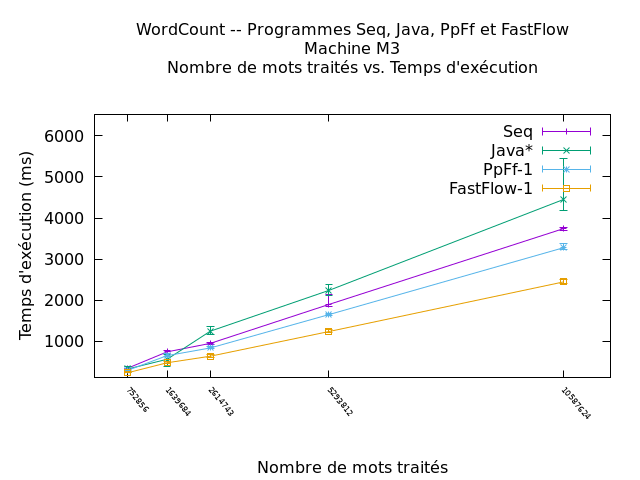
\includegraphics[width=1.0\textwidth]{Figures/WordCount-temps-c34581-400-30.png}
%      \caption[Les temps d'ex\'ecution pour \TT{WordCount} sur la machine \M3.]{Les temps d'ex\'ecution pour \TT{WordCount} sur la machine \M3, pour les programmes \TT{Seq}, \TT{Java}, \TT{PpFf} et \TT{FastFlow}. Les temps sont en millisecondes (ms), obtenus en prenant la moyenne de 30 ex\'ecutions.}
%       \label{GrapheTempsWordCountLinux.fig}
%\end{figure}
%
%\begin{figure}
%\centering
%     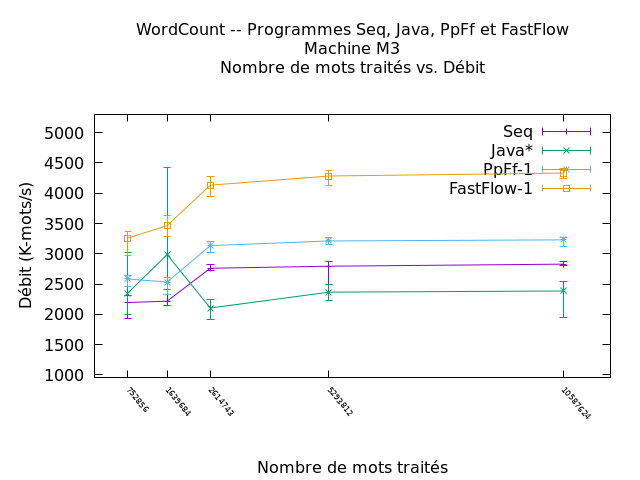
\includegraphics[width=1.0\textwidth]{Figures/WordCount-debits-c34581-400-30.png}
%      \caption[Les d\'ebits pour \TT{WordCount} sur la machine \M3.]{Les d\'ebits pour \TT{WordCount} sur la machine \M3, pour les programmes \TT{Seq}, \TT{Java}, \TT{PpFf} et \TT{FastFlow}. Les d\'ebits sont en milliers de mots par seconde (K-mots/s), obtenus en prenant la moyenne de 30 ex\'ecutions.}
%       \label{GrapheDebitsWordCountLinuxt.fig}
%\end{figure}

Dans cette section, nous 
% présentons une \'evaluation exp\'erimentale approfondie pour les op\'erations d\'ecrites dans la section pr\'ec\'edente. Nous
\'evaluons l'application \TT{WordCount} en examinant le temps d'ex\'ecution requis en fonction du nombre de mots. Afin de conna\^itre l'impact de la quantit\'e de donn\'ees \`a traiter, les exp\'eriences ont \'et\'e men\'ees en utilisant plusieurs ensembles de donn\'ees. Chaque ensemble de donn\'ees --- un fichier sur disque --- contient un nombre croissant de mots. Ces nombres de mots varient de 78~792 \`a 2~614~743. Pour toutes les exp\'eriences, le facteur de r\'ep\'etitions a \'et\'e \'etabli \`a 10.  Les r\'esultats sont pr\'esent\'es dans les figures~\ref{GrapheTempsWordCountJava.fig} et~\ref{GrapheTempsWordCountJapet.fig} respectivement: la figure~\ref{GrapheTempsWordCountJava.fig} montre les résultats obtenus sur la machine~\M1\ alors que la figure~\ref{GrapheTempsWordCountJapet.fig} montre ceux obtenus sur la machine M2.  Les deux axes des diagrammes sont interpr\'et\'es \`a l'aide des deux m\'etriques suivantes : le nombre de mots trait\'es est indiqu\'e sur l'axe des $x$, alors que le temps d'ex\'ecution r\'esultant est indiqu\'e sur l'axe des $y$.  Soulignons qu'afin de visualiser l'ensemble des exp\'eriences (nombres de mots trait\'es) sur une m\^eme figure, l'\'echelle pour le temps d'ex\'ecution est \emph{logarithmique}. 

Deux s\'eries d'exp\'eriences ont \'et\'e men\'ees dans le cas de \TT{Java}. L'une avec \emph{JIT} et l'autre sans. Les r\'esultats de ces exp\'eriences sont marqu\'es dans les deux diagrammes par \TT{Java+} et \TT{Java-} respectivement. Dans le cas de \TT{PpFf}, les exp\'eriences ont \'et\'e men\'ees en variant les nombres de \emph{threads}. Deux \emph{threads} ont \'et\'e utilis\'es sur la machine \M1\ et huit sur la machine \M2. Le suffixe de type entier dans les notations de \TT{PpFf} de deux diagrammes repr\'esente le nombre de \emph{threads} utilis\'es dans les exp\'eriences. Par exemple pour \TT{PpFf-2}, deux \emph{threads} ont \'et\'e utilis\'es et pour \TT{PpFf-4}, quatre \emph{threads} ont \'et\'e utilis\'es.



Les exp\'eriences men\'ees sur la machine \M1\ montrent que le temps d'ex\'ecution de \TT{Java} sans \TT{JIT} est nettement sup\'erieur \`a celui avec \TT{JIT}. Dans le cas de \TT{PpFf}, le temps d'ex\'ecution avec un \emph{thread} par rapport \`a celui avec deux \emph{threads} est meilleur lorsque la charge du travail est petite. Cela peut s'expliquer par les surco\^uts suppl\'ementaires introduits par la cr\'eation de \emph{threads}.

En comparant les temps d'ex\'ecutions entre \TT{PpFf} et \TT{Java}, on constate que, pour une petite charge de travail, \TT{PpFf} obtient de meilleurs temps d'ex\'ecution. Lorsque la charge du travail augmente, \TT{Java} se comporte mieux. Cela peut \^etre observ\'e dans la figure~\ref{GrapheTempsWordCountJava.fig}, o\`u \TT{Java} obtient de meilleurs temps d'ex\'ecution par rapport \`a \TT{PpFf--1}. 

La gestion de \emph{threads} entre les deux programmes diff\`ere. \TT{PpFf} ex\'ecute chaque op\'eration d'un \TT{pipeline} sur un \emph{thread} diff\'erent. Par exemple, les cinq op\'erations de \TT{WordCount} --- \TT{source}, \TT{flatMap}, \TT{map}, \TT{find} et \TT{reduceByKey} --- s'ex\'ecutent sur cinq \emph{threads} diff\'erents. Par contre, \TT{Java} g\`ere la cr\'eation de \emph{threads} par l'interm\'ediaire du \emph{framework} \TT{fork/join}. D\'ecrit dans le chapitre~\ref{outils_connus.chap} (p.~\pageref{forkjoin.sect}), le \emph{framework} divise une t\^ache en plus petites sous-t\^aches ind\'ependantes, et ce r\'ecursivement jusqu'\`a ce qu'elles soient assez simples pour \^etre ex\'ecut\'ees. Ce m\'ecanisme permet \`a \TT{Java} d'\^etre plus efficace que \TT{PpFf--1}. \TT{PpFf} est plus rapide que \TT{Java} lorsqu'on augmente le nombre de \emph{threads}. On peut observer cela dans la figure~\ref{GrapheTempsWordCountJava.fig}. \TT{PpFf--2} obtient de meilleurs temps d'ex\'ecution que \TT{Java} pour une charge de travail plus grande.

Les m\^emes exp\'eriences ont \'et\'e men\'ees sur la machine \M2. Par rapport \`a la machine \M1\, \M2\ dispose de plusieurs processeurs. Cela nous a permis d'ex\'ecuter plusieurs s\'eries d'exp\'eriences en faisant varier le nombre de \emph{threads} dans le programme \TT{PpFf}. La figure~\ref{GrapheTempsWordCountJapet.fig} montre les r\'esultats obtenus pour les deux programmes. On peut constater que \TT{PpFf} obtient de meilleurs temps d'ex\'ecution  que \TT{Java}. 


\begin{center}
\footnotesize
\begin{longtable}{|r|r|r|}
\caption{Le nombre de mots trait\'es par unit\'e de temps pour~\PpFf-2 sur la machine~\M2.\label{experiencesPpFf2.tab}}\\
\hline
\textbf{Nb.\ de mots} & \textbf{Temps ex\'ec.\ (ms)} & \textbf{D\'ebit (nb.\ mots/ms)}\\
\hline
\endfirsthead
\multicolumn{3}{c}%
{\tablename\ \thetable\ Les méthodes publiques de l'API (\textit{suite})} \\
\hline
\textbf{M\'ethode} & \textbf{Type du r\'esultat} & \textbf{Description du r\'esultat}\\
\hline
\endhead
\hline \multicolumn{3}{r}{\textit{Suite page suivante}} \\
\endfoot
\hline
\endlastfoot
\hline
	78~792 &
	151 & 
    522
    \\
\hline
	167~941 &
	291 & 
    577
    \\ 
\hline
	281~307 &
	474 & 
    593
    \\ 
\hline
	482~636 &
	793 & 
    609
    \\ 
\hline
	752~856 &
	1~263 & 
    596
    \\ 
\hline
	1~639~684 &
	2~724 & 
    602
    \\ 
\hline
	2~137~758 &
	4~124 & 
    518
    \\ 
\hline
	2~614~743 &
	4~724 & 
    554
    \\                      
\hline    
\end{longtable}
\normalsize
\end{center}    

Un point int\'eressant, qui peut \^etre observ\'e dans ce diagramme, est que le temps total d'ex\'ecution augmente de fa\c {c}on \emph{lin\'eaire} en fonction du nombre de mots trait\'es. En prenant comme exemple le diagramme pour \TT{PpFf-2} de la figure~\ref{GrapheTempsWordCountJapet.fig}, le tableau~\ref{experiencesPpFf2.tab} pr\'esente le nombre de mots trait\'es, le temps d'ex\'ecution et le d\'ebit --- nombre de mots trait\'es par ms --- pour~\TT{PpFf-2} sur la machine~\M2.  On peut noter que pour la plus petite charge de travail, \TT{PpFf} traite 522 mots/ms et 554 mots/ms pour le plus gros fichier, et que le d\'ebit reste relativement stable peu importe la taille du fichier. Cela d\'emontre que \TT{PpFf} est efficace non seulement pour un petit volume de travail, mais aussi pour de grands traitements de donn\'ees.  



\section{Analyse de l'application \TT{StockPrice}}
\label{stockprice.sect}

Dans le monde informatique actuel, les institutions financi\`eres produisent d'\'enormes quantit\'es d'informations, par ex., des informations sur les march\'es boursiers. Un probl\`eme important qu'elles rencontrent consiste \`a trouver des moyens efficaces pour r\'esumer et visualiser les donn\'ees afin de produire des informations utiles sur le comportement du march\'e, notamment pour prendre des d\'ecisions d'investissement. Cette section pr\'esente une application qui calcule le prix maximum pour diverses actions d'un marché boursier. Le code source des applications \TT{StockPrice} en \TT{PpFf} et~\TT{Java} est pr\'esent\'e dans les annexes~\ref{sourceCodeStockPricePpFf.ann} et~\ref{sourceCodeStockPriceJava.ann} respectivement. 

\subsection{Description de l'application}

L'application \TT{StockPrice} calcule le prix d'une action en utilisant le modèle \emph{Black-Scholes}~\citep{macbeth1979empirical}. Ce mod\`ele d'\'evaluation est utilis\'e pour d\'eterminer le prix juste ou la valeur th\'eorique d'une option d'achat ou de vente, et ce en fonction de six variables telles que la valeur de l'action sous-jacente, le prix d'exercice, le taux d'int\'er\^et sans risque, la volatilit\'e du prix de l'action, la dur\'ee et le type d'option. 

L'application \TT{StockPrice} est compos\'ee de cinq op\'erations principales~: 

\begin{lstlisting}[
label={exampleInfoActionFromFile},
language=c++,
caption={Un exemple illustrant l'information sur des actions contenues dans le fichier.},
frame=single,
float]
SNY 100.00 90.00 0.1000 0.00 0.10 1.00 C 0.00 18.6308591206674982
JCI 100.00 100.00 0.1000 0.00 0.10 0.50 C 0.00 5.8502736042849798
DSX 100.00 100.00 0.1000 0.00 0.10 1.00 C 0.00 10.3081472436668
LILA 100.00 110.00 0.1000 0.00 0.10 0.10 C 0.00 0.003523074865
NVS 100.00 110.00 0.1000 0.00 0.10 0.50 C 0.00 1.1407228438274099
FLML 100.00 110.00 0.1000 0.00 0.10 1.00 C 0.00 4.216747020308
TEF 100.00 90.00 0.1000 0.00 0.25 0.10 C 0.00 11.1352446183467002
DXB 100.00 90.00 0.1000 0.00 0.25 0.50 C 0.00 16.0926388440922991
HSEA 100.00 90.00 0.1000 0.00 0.25 1.00 C 0.00 21.16345465848
LENS 100.00 100.00 0.1000 0.00 0.25 0.10 C 0.00 3.65996266031
\end{lstlisting}

\begin{itemize}

\item Une op\'eration qui d\'efinit la source du flux de donn\'ees. Ici, la source est constitu\'ee par les lignes contenues dans un fichier. Le listing~\ref{exampleInfoActionFromFile} montre un exemple avec quelques enregistrements tir\'es de notre fichier de test. 

Un enregistrement est identifi\'e par les informations suivantes : le nom de l'action, la valeur actuelle de l'action sous-jacente, le prix d'exercice, le taux d'int\'er\^et sans risque, le taux de dividende, la volatilit\'e du prix de l'action, le temps qu'il reste \`a l'option avant son \'ech\'eance (exprim\'e en ann\'ees), le type d'option (\TT{C=CALL}~: prix pour une option d'achat~; \TT{P=PUT}~: prix pour une option de vente), la valeur de dividende et la valeur de r\'ef\'erence \TT{DerivaGem}. 
Les valeurs \TT{DerivaGem}, la valeur et le taux de dividende ne sont pas utilis\'es dans \TT{StockPrice} pour calculer le prix d'une action.

\item Une op\'eration qui r\'epartit les \'el\'ements du flux entre divers \emph{threads}.
Toutes les \'etapes qui suivent cette op\'eration seront donc ex\'ecut\'ees en parall\`ele.

\item Une op\'eration  \TT{map}, qui permet d'extraire le nom et les options de chaque action.


\item  Une op\'eration qui calcule le prix de chaque action. L'algorithme utilis\'e est celui de \emph{Black-Scholes}~\citep{macbeth1979empirical}. 

\item Une derni\`ere op\'eration qui extrait le prix maximum pour chaque action.


\end{itemize}

\subsection{Mesures obtenues et analyse des r\'esultats}

\graphe{StockPrice-temps-java-700-30}{Programmes Seq, Java, PpFf et FastFlow}
\graphe{StockPrice-debits-java-700-30}{Programmes Seq, Java, PpFf et FastFlow}

\graphe{StockPrice-temps-japet-700-30}{Programmes Seq, Java, PpFf et FastFlow}
\graphe{StockPrice-debits-japet-700-30}{Programmes Seq, Java, PpFf et FastFlow}

\graphe{StockPrice-temps-c34581-400-30}{Programmes Seq, Java, PpFf et FastFlow}
\graphe{StockPrice-debits-c34581-400-30}{Programmes Seq, Java, PpFf et FastFlow}

%
%\begin{figure}
%\centering
%     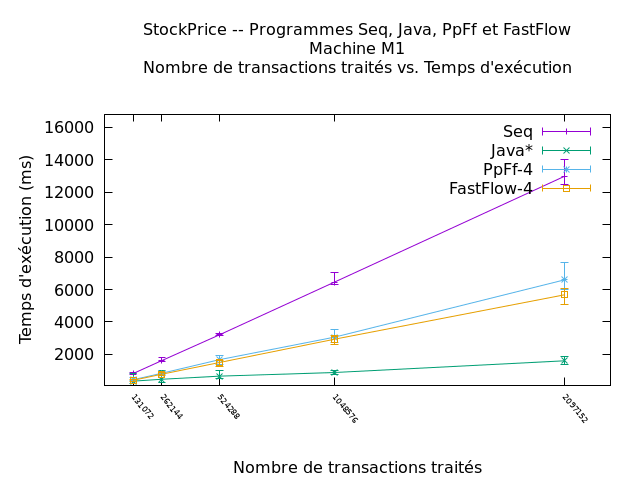
\includegraphics[width=1.0\textwidth]{Figures/StockPrice-temps-java-700-30.png}
%      \caption[Les temps d'ex\'ecution pour \TT{StockPrice} sur la machine \M1.]{Les temps d'ex\'ecution pour \TT{StockPrice} sur la machine \M1, pour les programmes \TT{Seq}, \TT{Java}, \TT{PpFf} et \TT{FastFlow}. Les temps sont en millisecondes (ms), obtenus en prenant la moyenne de 30 ex\'ecutions.}
%       \label{GrapheTempsStockPriceJava.fig}
%\end{figure}
%
%\begin{figure}
%\centering
%     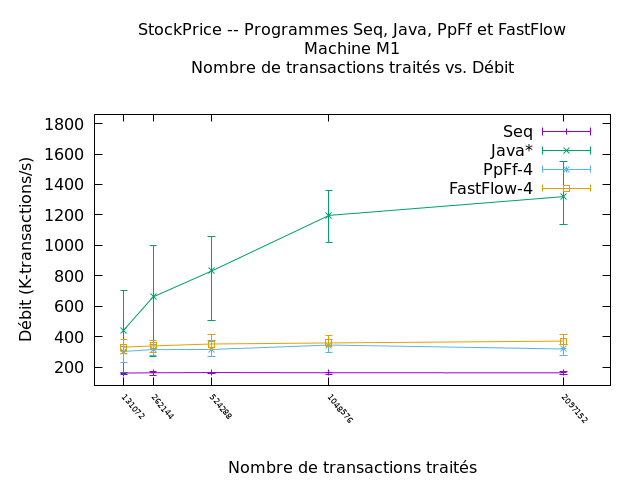
\includegraphics[width=1.0\textwidth]{Figures/StockPrice-debits-java-700-30.png}
%      \caption[Les d\'ebits pour \TT{StockPrice} sur la machine \M1.]{Les d\'ebits pour \TT{StockPrice} sur la machine \M1, pour les programmes \TT{Seq}, \TT{Java}, \TT{PpFf} et \TT{FastFlow}. Les d\'ebits sont en milliers de mots par seconde (K-mots/s), obtenus en prenant la moyenne de 30 ex\'ecutions.}
%       \label{GrapheDebitsStockPriceJava.fig}
%\end{figure}
%
%\begin{figure}
%\centering
%     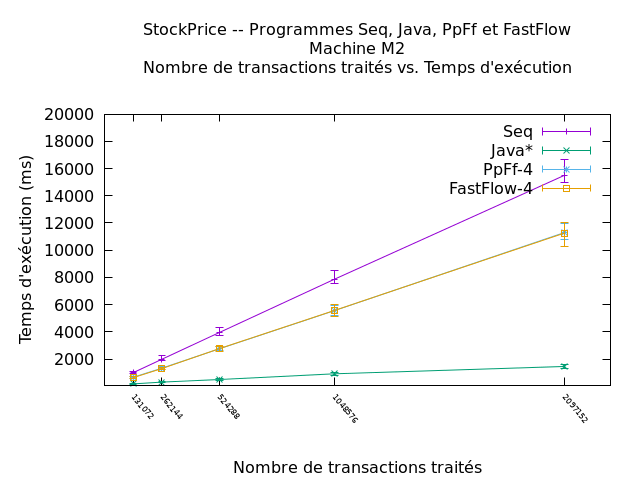
\includegraphics[width=1.0\textwidth]{Figures/StockPrice-temps-japet-700-30.png}
%      \caption[Les temps d'ex\'ecution pour \TT{StockPrice} sur la machine \M2.]{Les temps d'ex\'ecution pour \TT{StockPrice} sur la machine \M2, pour les programmes \TT{Seq}, \TT{Java}, \TT{PpFf} et \TT{FastFlow}. Les temps sont en millisecondes (ms), obtenus en prenant la moyenne de 30 ex\'ecutions.}
%       \label{GrapheTempsStockPriceJapet.fig}
%\end{figure}
%
%\begin{figure}
%\centering
%     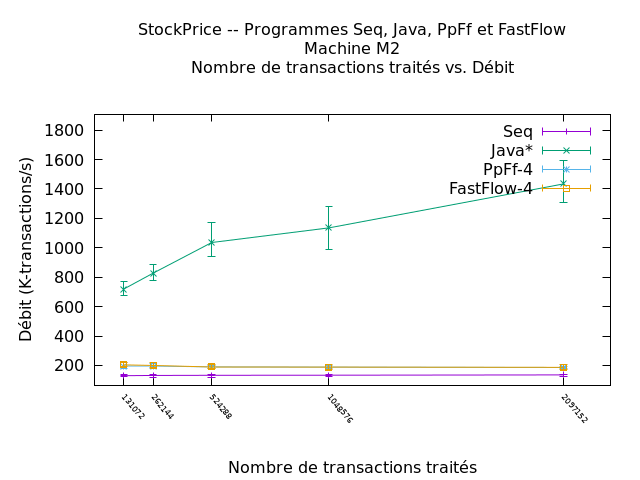
\includegraphics[width=1.0\textwidth]{Figures/StockPrice-debits-japet-700-30.png}
%      \caption[Les d\'ebits pour \TT{StockPrice} sur la machine \M2.]{Les d\'ebits pour \TT{StockPrice} sur la machine \M2, pour les programmes \TT{Seq}, \TT{Java}, \TT{PpFf} et \TT{FastFlow}. Les d\'ebits sont en milliers de mots par seconde (K-mots/s), obtenus en prenant la moyenne de 30 ex\'ecutions.}
%       \label{GrapheDebitsStockPriceJapet.fig}
%\end{figure}
%
%\begin{figure}
%\centering
%     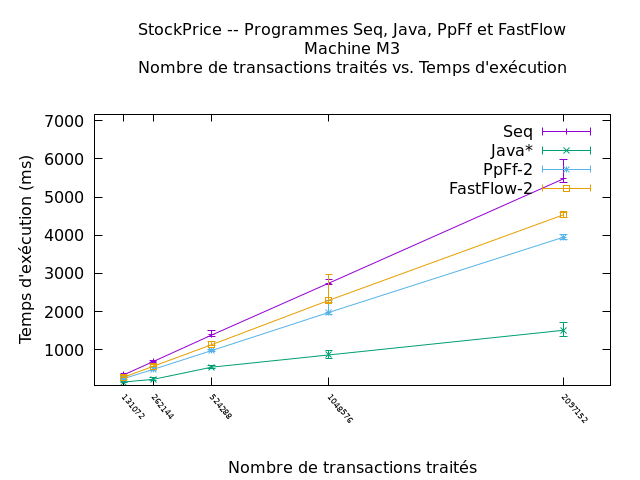
\includegraphics[width=1.0\textwidth]{Figures/StockPrice-temps-c34581-400-30.png}
%      \caption[Les temps d'ex\'ecution pour \TT{StockPrice} sur la machine \M3.]{Les temps d'ex\'ecution pour \TT{StockPrice} sur la machine \M3, pour les programmes \TT{Seq}, \TT{Java}, \TT{PpFf} et \TT{FastFlow}. Les temps sont en millisecondes (ms), obtenus en prenant la moyenne de 30 ex\'ecutions.}
%       \label{GrapheTempsStockPriceLinux.fig}
%\end{figure}
%
%\begin{figure}
%\centering
%     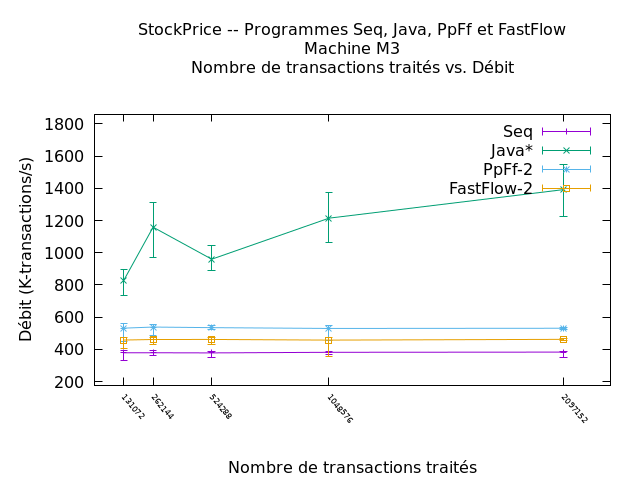
\includegraphics[width=1.0\textwidth]{Figures/StockPrice-debits-c34581-400-30.png}
%      \caption[Les d\'ebits pour \TT{StockPrice} sur la machine \M3.]{Les d\'ebits pour \TT{StockPrice} sur la machine \M3, pour les programmes \TT{Seq}, \TT{Java}, \TT{PpFf} et \TT{FastFlow}. Les d\'ebits sont en milliers de mots par seconde (K-mots/s), obtenus en prenant la moyenne de 30 ex\'ecutions.}
%       \label{GrapheDebitsStockPriceLinuxt.fig}
%\end{figure}
%


Les r\'esultats  pour l'application \TT{StockPrice} sont pr\'esent\'es dans la figure~\ref{executionTimesStockPrice.fig}. Les expériences ont aussi \'et\'e menées sur les deux machines \M1 et~\M2 et les temps d'ex\'ecution pour \ppff\ et \TT{Java} sont indiqu\'es sur la m\^eme figure --- gauche: \M1, droite: \M2. 
%
%\IC{J'ai ajout\'e des d\'etails concernant les \emph{threads} utilis\'es par \ppff.}
Dans le cas de \ppff\, plusieurs exp\'eriences ont \'et\'e men\'ees en variant le nombre de \emph{threads}. La figure~\ref{executionTimesStockPrice.fig} montre le meilleur temps d'ex\'ecution obtenu par celui-ci sur les deux machines. La meilleure performance sur la machine \M1\ a \'et\'e obtenue avec deux \emph{threads} et avec quatre sur la machine \M2.
%
Chaque programme calcule le prix maximum pour plusieurs actions. Le temps d'ex\'ecution r\'esultant est repr\'esent\'e sur l'axe des $y$ de la figure~\ref{executionTimesStockPrice.fig}. 

On remarque que dans les deux cas, \TT{PpFf} obtient de meilleurs temps d'ex\'ecution en comparaison avec \TT{Java}. Sur la machine \M1, \TT{PpFf} est plus de 7 fois plus rapide que \TT{Java}. Tandis que \TT{PpFf} trouve le prix maximum de l'action en seulement 232~ms, Java requiert 1~629~ms pour la m\^eme t\^ache. Un meilleur temps d'ex\'ecution est obtenu par \TT{Java} sur la machine \M2 que sur la machine \M1. Avec un temps d'ex\'ecution de 411~ms, \TT{Java} est presque 4 fois plus rapide en comparaison avec le m\^eme programme \TT{Java} sur la machine \M1. Toutefois, m\^eme si \TT{Java} se comporte mieux sur cette machine, son temps d'ex\'ecution n'est pas meilleur que celui de \TT{PpFf}. Avec 304~ms, \TT{PpFf} est toujours plus rapide que \TT{Java}. 





%
%\section{Analyse des surco\^uts de \TT{PpFf} par rapport \`a \TT{FastFlow}}
%\label{coutsPpFf.sect}
%
%Tel que d\'ecrit dans le chapitre~\ref{implementation.chap}, \TT{PpFf} est impl\'ement\'e au-dessus de la biblioth\`eque \TT{FastFlow}. Cette section examine les surco\^uts introduits par \TT{PpFf} par rapport \`a \TT{FastFlow}. 
%
%\subsection{Description de l'application}
%
%Pour cette exp\'erience, nous avons cr\'e\'e un \emph{micro benchmark} consistant en un {pipeline} avec un seul op\'erateur. L'op\'erateur choisi pour cette exp\'erience est un \TT{map} qui fait un simple calcul it\'eratif, plus pr\'ecis\'ement qui incr\'emente  \TT{nb} fois une variable \TT{*res}, avec~\TT{nb}~=~$10^{\TT{granularity}}$~:
%{
%\begin{lstlisting}[language=c++]
%  int nb = pow(10, granularity);
%  for (int i = 1; i <= nb; i++) {
%    *res += 1;   
%  }
%\end{lstlisting}
%} 
%
%Ici, \TT{granularity} est un param\`etre sp\'ecifi\'e en argument lors du lancement de l'application. Le code source de cette application pour~\TT{PpFf} et~\TT{FastFlow} est pr\'esent\'e en annexe (Annexes~\ref{sourceCodeMicrobenchmarkPpFf.ann} et~\ref{sourceCodeMicrobenchmarkFastFlow.ann} respectivement). Le m\^eme calcul se r\'ep\`ete pour chaque \'el\'ement dans le pipeline, o\`u la source est constitu\'ee d'une suite d'\'el\'ements. Plus sp\'ecifiquement, pour cette exp\'erience, la suite est compos\'ee des entiers allant de 1 \`a 100~000.  
%
%
%\subsection{Mesures obtenues et analyse des r\'esultats}
%
%Afin d'identifer les surco\^uts introduits par \PpFf{} par rapport \`a \TT{FastFlow}, deux s\'eries d'exp\'eriences ont \'et\'e men\'ees~: une avec \TT{granularity = 4}, l'autre avec \TT{granularity~=~5}. Pour la suite d'entiers allant de 1 \`a 100~000, les exp\'eriences ont \'et\'e r\'ealis\'ees avec un nombre variable de \emph{threads} sur deux machines diff\'erentes : \M1\ et \M2.  
%
%
%\begin{figure}
%\centering
%     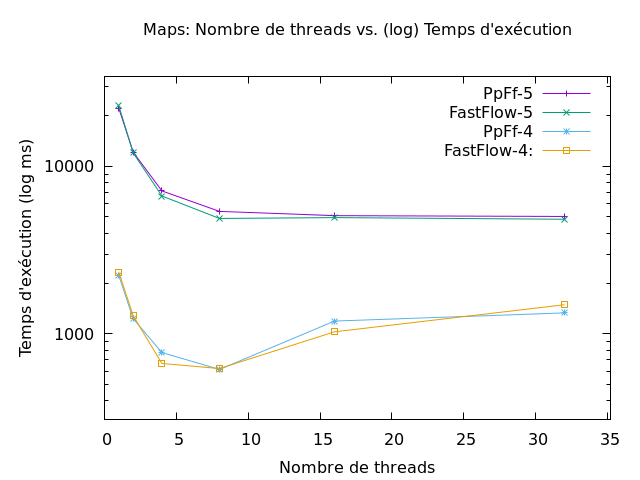
\includegraphics[width=1.0\textwidth]{Figures/graphe_temps_Java_Maps.png}
%      \caption{Les temps d'ex\'ecution pour \TT{MicroBenchmarkMaps} sur la machine \M1.}
%       \label{GrapheTempsMapsJava.fig}
%\end{figure}
%
%\begin{figure}
%\centering
%     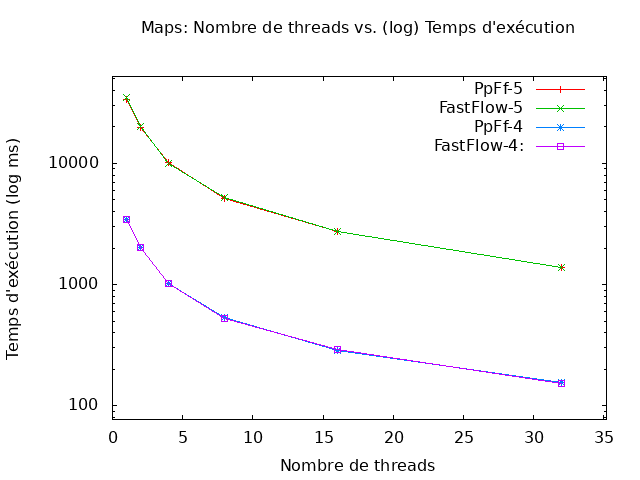
\includegraphics[width=1.0\textwidth]{Figures/graphe_temps_Japet_Maps.png}
%      \caption{Les temps d'ex\'ecution pour \TT{MicroBenchmarkMaps} sur la machine \M2.}
%       \label{GrapheTempsMapstJapet.fig}
%\end{figure}
%
%
%La figure~\ref{GrapheTempsMapsJava.fig} montre les r\'esultats des exp\'eriences sur la machine \M1\ alors que la figure~\ref{GrapheTempsMapstJapet.fig} montre les r\'esultats des exp\'eriences sur la machine \M2. On constate un faible surco\^ut
%introduit par \TT{PpFf} sur la machine \M1. Ce surco\^ut est plus \'evident lorsque la surcharge du calcul est moins grande. Pourtant, les surco\^uts introduits par \TT{PpFf} par rapport \`a \TT{FastFlow} restent faibles --- c'est ce qui explique, surtout dans la figure~\ref{GrapheTempsMapstJapet.fig}, que les lignes du graphe pour \TT{PfFf} et \TT{FastFlow}, tant avec 4 que 5 \emph{threads}, soient quasiment identiques~: la plus grande diff\'erence entre les temps d'ex\'ecutions de deux applications est de 300~ms. Le volume de traitement des deux applications est tr\`es grand. Le pipeline traite 100~000 \'el\'ements et l'algorithme de calcul appliqu\'e \`a chaque \'el\'ement consiste \`a incr\'ementer une valeur de 0 \`a 10~000 dans le cas avec la granularit\'e 4, ou de 0 \`a 100~000 avec la granularit\'e 5. Or, en prenant en consid\'eration ce grand volume de traitement des deux applications, ces 300~ms semblent n\'egligeables.

